\documentclass[a4paper, 11pt]{article}

% --- Geometry & Margins ---
\usepackage[top=0.85in, bottom=0.85in, left=0.9in, right=0.9in]{geometry}
\usepackage{times}
\usepackage{setspace}
\onehalfspacing

% --- Math & Symbols ---
\usepackage{amsmath, amssymb, amsfonts, bm}

% --- Tables & Arrays ---
\usepackage{booktabs}
\usepackage{tabularx}
\usepackage{multirow}
\usepackage{array}

% --- Colors & Graphics ---
\usepackage{xcolor}
\usepackage{graphicx}
\usepackage{float}

% --- Framing & Boxes ---
\usepackage[most]{tcolorbox}

% --- Header, Footer & Lists ---
\usepackage{fancyhdr}
\usepackage{enumitem}
\setlist{noitemsep, topsep=3pt}

% --- Hyperlinks ---
\usepackage[colorlinks=true, linkcolor=blue!70!black, urlcolor=blue!70!black, citecolor=blue!70!black]{hyperref}

% --- Colors Palette ---
\definecolor{primaryblue}{RGB}{20, 45, 110}
\definecolor{secondaryblue}{RGB}{41, 128, 185}
\definecolor{accentdark}{RGB}{44, 62, 80}
\definecolor{techbg}{RGB}{245, 248, 255}
\definecolor{techborder}{RGB}{41, 128, 185}
\definecolor{tipbg}{RGB}{254, 249, 231}
\definecolor{tipborder}{RGB}{243, 156, 18}
\definecolor{defensebg}{RGB}{253, 245, 245}
\definecolor{defenseborder}{RGB}{192, 57, 43}
\definecolor{eqbg}{RGB}{248, 249, 250}
\definecolor{eqborder}{RGB}{149, 165, 166}

% --- Custom Boxes ---
\newtcolorbox{techbox}[2][]{%
  enhanced,
  colback=techbg,
  colframe=techborder,
  arc=2.5mm,
  boxrule=1pt,
  fonttitle=\bfseries\color{white},
  coltitle=white,
  colbacktitle=primaryblue,
  title={#2},
  attach boxed title to top left={yshift=-2mm, xshift=4mm},
  boxed title style={arc=1.5mm, boxrule=0pt, colback=primaryblue},
  top=4mm, bottom=3mm, left=4mm, right=4mm,
  breakable,
  #1
}

\newtcolorbox{defensebox}[2][]{%
  enhanced,
  colback=defensebg,
  colframe=defenseborder,
  arc=2.5mm,
  boxrule=1pt,
  fonttitle=\bfseries\color{white},
  coltitle=white,
  colbacktitle=defenseborder,
  title={#2},
  attach boxed title to top left={yshift=-2mm, xshift=4mm},
  boxed title style={arc=1.5mm, boxrule=0pt, colback=defenseborder},
  top=4mm, bottom=3mm, left=4mm, right=4mm,
  breakable,
  #1
}

\newtcolorbox{tipbox}[1][Viva Defense Strategy]{%
  enhanced,
  colback=tipbg,
  colframe=tipborder,
  arc=2mm,
  boxrule=0.8pt,
  fonttitle=\bfseries\color{tipborder!80!black},
  title={#1},
  top=2mm, bottom=2mm, left=3mm, right=3mm,
  breakable
}

\newtcolorbox{cheatsheetbox}[1][Quick Memorization Card]{%
  enhanced,
  colback=white,
  colframe=accentdark,
  arc=2mm,
  boxrule=0.8pt,
  fonttitle=\bfseries\color{white},
  colbacktitle=accentdark,
  title={#1},
  top=2mm, bottom=2mm, left=3mm, right=3mm,
  breakable
}

% --- Header & Footer ---
\pagestyle{fancy}
\fancyhf{}
\fancyhead[L]{\small\textsf{\color{gray}Tribhuvan University (IoST) — Master's Thesis Defense Guide}}
\fancyhead[R]{\small\textsf{\color{gray}Architecture Deep-Dive: V-JEPA 2.1 vs. Qwen2.5-VL}}
\fancyfoot[C]{\thepage}
\renewcommand{\headrulewidth}{0.4pt}
\renewcommand{\footrulewidth}{0.4pt}

% =============================================================================
\begin{document}

% --- Title Banner ---
\begin{center}
  {\fontsize{18}{22}\selectfont \textbf{\color{primaryblue}DEEP ARCHITECTURAL GUIDE \& DEFENSE MASTERCLASS}}\\[3pt]
  {\fontsize{13}{16}\selectfont \textbf{\color{accentdark}V-JEPA 2.1 vs. Qwen2.5-VL for Video Action Recognition}}\\[3pt]
  {\fontsize{10}{13}\selectfont Prepared for Master of Science in Information Technology (M.Sc. IT / MIT) Thesis Defense}\\[2pt]
  {\fontsize{10}{13}\selectfont Central Department of Computer Science \& Information Technology (CDCSIT), IoST, Tribhuvan University, Nepal}\\[6pt]
  \rule{\textwidth}{1.2pt}\\[5pt]
  {\fontsize{10}{13}\selectfont \textbf{Thesis Title:} \textit{Enhancing Self-Supervised Video Representations with HAF-STD Net:}}\\
  {\fontsize{10}{13}\selectfont \textit{A Comparative Evaluation Against VLM for Action Recognition}}\\[5pt]
  \textbf{Candidate:} Erize Rai \quad$|$ \quad \textbf{Roll No:} 8025006 \quad$|$ \quad \textbf{Reg. No:} 5-3-28-193-2023\\
  \textbf{Supervisor:} Asst. Prof. Dr. Dhiraj Kedar Pandey\\[2pt]
  \rule{\textwidth}{0.6pt}
\end{center}

\vspace{0.2cm}
\tableofcontents
\newpage

% =============================================================================
\section{Executive Overview: Why This Matters for Your Defense}
% =============================================================================

In your thesis defense, the committee will scrutinize the foundational premises of your comparative study. Your research juxtaposes two fundamentally distinct paradigms in modern visual representation learning:
\begin{enumerate}
    \item \textbf{V-JEPA 2.1 (Meta AI, 654M parameters):} A non-generative, self-supervised video foundation model trained entirely in \emph{latent representation space} through masked spatiotemporal prediction without text guidance or pixel reconstruction.
    \item \textbf{Qwen2.5-VL (Alibaba Cloud, 7B parameters):} A multimodal autoregressive vision-language model trained jointly on massive image-text-video corpora, equipped with dynamic-resolution vision encoding and causal language decoding.
\end{enumerate}

\begin{tipbox}[The Core Defense Thesis Argument]
Your key empirical finding is that \textbf{V-JEPA 2.1 paired with HAF-STD Net achieves 98.1\% accuracy (97.8\% macro F1) on FineGym and 84.7\% accuracy (85.3\% macro F1) on HMDB51}, outperforming Qwen2.5-VL (88.4\% F1 on FineGym, 79.1\% F1 on HMDB51) by substantial margins (+9.4\% and +6.2\% F1), despite V-JEPA 2.1 having \textbf{$\sim$10$\times$ fewer parameters} (654M vs. 7B).

\emph{Examiners will ask:} ``Why does a model with 10$\times$ fewer parameters beat an advanced 7B vision-language foundation model?'' This document equips you with the exact architectural, mathematical, and representational answers to dominate that question.
\end{tipbox}

\vspace{0.3cm}

% =============================================================================
\section{Architecture 1: V-JEPA 2.1 (Meta AI)}
% =============================================================================

\subsection{Foundational Concept: The JEPA Paradigm}
Traditional self-supervised vision methods rely on one of two paradigms:
\begin{itemize}
    \item \textbf{Generative / Pixel-level Reconstruction (MAE, VideoMAE):} Predict missing pixels $x \in \mathbb{R}^3$. \emph{Flaw:} Forces the network to waste capacity modeling high-frequency unpredictable noise (foliage texture, lighting fluctuations, background static) rather than high-level semantic dynamics.
    \item \textbf{Contrastive Learning (SimCLR, MoCo):} Push augmented views together while pushing negative samples apart. \emph{Flaw:} Requires delicate negative sample mining, large batch sizes, and heavy handcrafted data augmentations that can alter physical motion semantics.
\end{itemize}

\textbf{Joint Embedding Predictive Architecture (JEPA)}, proposed by Yann LeCun, eliminates both drawbacks: it predicts the \emph{representation of masked regions in a learned latent feature space}. Because the loss is calculated in feature space, the encoder is free to discard low-level pixel noise and retain only semantic spatiotemporal structure.

\begin{figure}[H]
\centering
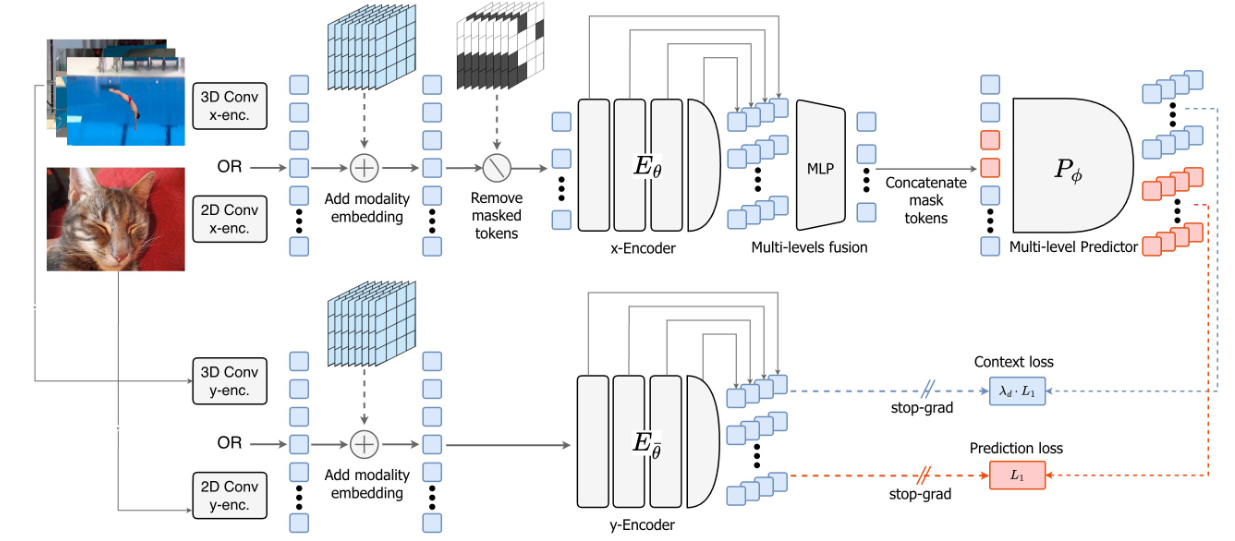
\includegraphics[width=0.92\textwidth]{fig/vjepa2.png}
\caption{Architecture of V-JEPA 2.1 self-supervised pretraining framework: dual x-Encoder and y-Encoder pipeline with multi-level intermediate fusion, mask-denoising predictor, and stop-gradient EMA targets.}
\label{fig:vjepa2_diagram}
\end{figure}

\subsection{Step-by-Step Architectural Pipeline of V-JEPA 2.1}

\subsubsection{1. Spatiotemporal Tokenization (3D Tubelet Convolution)}
Given an input video clip $\mathbf{V} \in \mathbb{R}^{B \times T \times H \times W \times C}$ ($T=8$ frames, $H=W=224$, $C=3$ channels):
\begin{itemize}
    \item Non-overlapping spatiotemporal \emph{tubelets} of size $2 \times 16 \times 16$ (temporal $\times$ height $\times$ width) are extracted using a 3D convolution layer with kernel size $(2, 16, 16)$ and stride $(2, 16, 16)$.
    \item Temporal token count: $T' = \frac{T}{2} = \frac{8}{2} = 4$.
    \item Spatial token grid: $H' = \frac{224}{16} = 14$, $W' = \frac{224}{16} = 14$.
    \item Total tokens per clip: $N = T' \times H' \times W' = 4 \times 14 \times 14 = 784$ tokens.
    \item Each tubelet is projected into hidden dimension $D = 1280$ (Vision Transformer Huge / ViT-H):
    \begin{equation}
        \mathbf{z}_0 = \text{Conv3D}(\mathbf{V}) + \mathbf{E}_{\text{3D-RoPE}}, \quad \mathbf{z}_0 \in \mathbb{R}^{B \times 784 \times 1280}
    \end{equation}
\end{itemize}

\subsubsection{2. 3D Rotary Position Embeddings (3D-RoPE)}
Unlike standard sinusoidal 1D position encodings that treat video as an unrolled sequence, V-JEPA 2.1 injects 3D coordinates $(t, h, w)$ directly into query-key attention matrices using rotary transformations:
\begin{equation}
    \mathbf{q}_m^T \mathbf{k}_n = (\mathbf{R}_{\Theta, m}^{3D} \mathbf{W}_q \mathbf{x}_m)^T (\mathbf{R}_{\Theta, n}^{3D} \mathbf{W}_k \mathbf{x}_n) = \mathbf{x}_m^T \mathbf{W}_q^T \mathbf{R}_{\Theta, n-m}^{3D} \mathbf{W}_k \mathbf{x}_n
\end{equation}
This preserves exact relative spatiotemporal distances across both spatial planes and temporal trajectories.

\subsubsection{3. Context Encoder \texorpdfstring{$E_\theta$}{E\_theta} (x-Encoder)}
\begin{itemize}
    \item \textbf{Backbone:} Vision Transformer Huge (ViT-H/16).
    \item \textbf{Parameters:} 654 Million.
    \item \textbf{Layers:} $L = 32$ Transformer blocks.
    \item \textbf{Attention Heads:} 16 heads, each of dimension $d_k = \frac{1280}{16} = 80$.
    \item \textbf{FFN Hidden Dimension:} $4 \times D = 5120$.
    \item \textbf{Precision:} Float16 with Scaled Dot-Product Attention (SDPA / FlashAttention).
    \item \textbf{Operation:} The context encoder processes the visible, unmasked spatiotemporal patches:
    \begin{equation}
        \mathbf{z}'_l = \text{MHSA}(\text{LN}(\mathbf{z}_{l-1})) + \mathbf{z}_{l-1}, \quad \mathbf{z}_l = \text{FFN}(\text{LN}(\mathbf{z}'_l)) + \mathbf{z}'_l
    \end{equation}
\end{itemize}

\subsubsection{4. Target Encoder \texorpdfstring{$E_{\bar{\theta}}$}{E\_theta\_bar} (y-Encoder) \& Exponential Moving Average (EMA)}
To supply target representations without collapsing to trivial constant representations:
\begin{itemize}
    \item The target encoder $E_{\bar{\theta}}$ shares the exact same ViT-H architecture as $E_\theta$.
    \item It processes the complete video view $y$.
    \item \textbf{CRITICAL DEFENSE POINT:} The target encoder receives \textbf{NO gradient descent updates} ($\nabla_{\bar{\theta}} \mathcal{L} = 0$). Its weights are updated strictly via Exponential Moving Average (EMA):
    \begin{equation}
        \bar{\theta} \leftarrow \tau \bar{\theta} + (1 - \tau) \theta, \quad \tau \in [0.996, 1.0)
    \end{equation}
    During pretraining, $\tau$ follows a cosine schedule starting at 0.996 and ramping up to 1.0.
\end{itemize}

\subsubsection{5. Predictor Network \texorpdfstring{$P_\phi$}{P\_phi}}
The predictor is a lightweight Vision Transformer (typically 12 layers, $D_{\text{pred}}=384$ or $512$). It receives:
\begin{itemize}
    \item The context representations $E_\theta(x)$ of visible patches.
    \item Learnable mask tokens $\Delta_y$ initialized with position embeddings representing target patch coordinates.
\end{itemize}
The predictor outputs predicted representations $\hat{s}_y = P_\phi(E_\theta(x), \Delta_y)$ for the masked target regions.

\subsubsection{6. Innovations in V-JEPA 2.1 vs. Previous V-JEPA Versions}
\begin{techbox}{Key Architectural Innovations of V-JEPA 2.1}
\begin{enumerate}
    \item \textbf{Dense Per-Token Latent Prediction Loss:} Rather than averaging representations across blocks, V-JEPA 2.1 computes token-by-token $L_1$ regression over all masked positions $M$:
    \begin{equation}
        \mathcal{L}_{\text{predict}} = \frac{1}{|M|} \sum_{i \in M} \left\| P_\phi(E_\theta(x), \Delta_y)_i - \operatorname{sg}(E_{\bar{\theta}}(y)_i) \right\|_1
    \end{equation}
    where $\operatorname{sg}(\cdot)$ is the stop-gradient operator.
    \item \textbf{Distance-Weighted Spatiotemporal Context Loss:} Enforces continuous spatial grounding by penalizing context representations near mask boundaries:
    \begin{equation}
        \mathcal{L}_{\text{context}} = \frac{1}{|C|} \sum_{j \in C} \lambda_d(j) \cdot \left\| E_\theta(x)_j - \operatorname{sg}(E_{\bar{\theta}}(y)_j) \right\|_1
    \end{equation}
    The total objective is: $\mathcal{L}_{\text{V-JEPA 2.1}} = \mathcal{L}_{\text{predict}} + \lambda_d \cdot \mathcal{L}_{\text{context}}$.
    \item \textbf{Multi-Layer Intermediate Supervision:} V-JEPA 2.1 applies predictive supervision not just to the 32nd layer, but across 4 intermediate depths: $\sim$25\% (layer 8), $\sim$50\% (layer 16), $\sim$75\% (layer 24), and 100\% (layer 32). This guarantees that middle layers contain rich semantic representations.
\end{enumerate}
\end{techbox}

\subsubsection{7. Multi-Layer Feature Extraction for HAF-STD Net}
In your thesis methodology, you exploit this multi-layer structure. Instead of simply pooling the final layer, you extract features from all 4 supervised intermediate depths:
\begin{equation}
    \mathbf{F}_{\text{multi}} = \left[\, \bar{\mathbf{z}}_{8};\; \bar{\mathbf{z}}_{16};\; \bar{\mathbf{z}}_{24};\; \bar{\mathbf{z}}_{32} \,\right] \in \mathbb{R}^{4 \times T' \times 1280} \quad (T'=4)
\end{equation}
where $\bar{\mathbf{z}}_l \in \mathbb{R}^{T' \times 1280}$ is the per-frame spatially mean-pooled token embedding at layer $l$. For baseline probes, global mean pooling over layer 32 yields a single vector $\mathbf{f} \in \mathbb{R}^{1280}$.

\vspace{0.3cm}

% =============================================================================
\section{Architecture 2: Qwen2.5-VL (Alibaba Cloud)}
% =============================================================================

\subsection{Foundational Concept: The Multimodal Autoregressive VLM}
Qwen2.5-VL (7B parameters) belongs to the family of Vision-Language Models (VLMs). Unlike V-JEPA's purely visual, self-supervised pretraining, Qwen2.5-VL is trained to align visual features with human language semantics through:
\begin{enumerate}
    \item Large-scale multimodal pretraining on billions of image-caption and video-text pairs.
    \item Visual instruction tuning on complex multimodal question-answering tasks.
    \item Autoregressive next-token prediction conditioned on visual tokens.
\end{enumerate}

\begin{figure}[H]
\centering
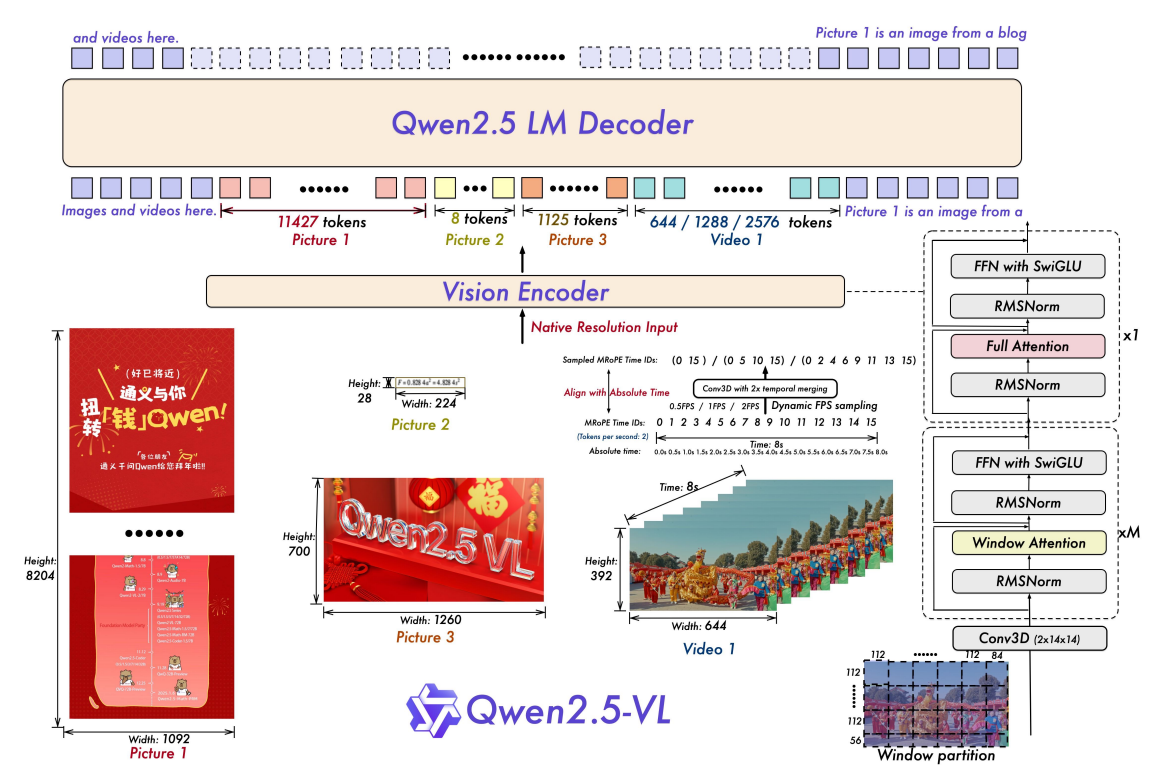
\includegraphics[width=0.92\textwidth]{fig/qwen.png}
\caption{Architecture of Qwen2.5-VL: Vision Encoder with Conv3D patch embedding and window attention feeding into the Qwen2.5 LM Decoder via an MLP merger with MRoPE alignment.}
\label{fig:qwen_diagram}
\end{figure}

\subsection{Step-by-Step Architectural Pipeline of Qwen2.5-VL}

\subsubsection{1. Native Dynamic Resolution Vision Encoder}
Traditional vision transformers resize all images/frames to a fixed square (e.g., $224 \times 224$), causing distortion, aspect-ratio skew, and blur. Qwen2.5-VL introduces \textbf{Native Dynamic Resolution}:
\begin{itemize}
    \item Input frames retain their original aspect ratio.
    \item Patches of size $14 \times 14$ pixels are extracted.
    \item For video inputs, a 3D convolution layer with temporal stride of 2 aggregates adjacent frames:
    \begin{equation}
        \mathbf{v}_0 = \text{Conv3D}(\mathbf{V}_{\text{frames}}), \quad \mathbf{v}_0 \in \mathbb{R}^{N_v \times D_v}
    \end{equation}
    where $N_v$ varies dynamically depending on the input video resolution.
\end{itemize}

\subsubsection{2. Window Attention Mechanism}
Because high-resolution video produces thousands of tokens ($N_v$), standard full self-attention would suffer quadratic computational complexity $\mathcal{O}(N_v^2)$. Qwen2.5-VL resolves this using \textbf{Window Attention}:
\begin{itemize}
    \item Tokens are partitioned into local spatial windows of size $w \times w$ (e.g., $112 \times 112$ pixels in patch coordinates).
    \item Self-attention is restricted within each window:
    \begin{equation}
        \text{WindowAttn}(\mathbf{Q}, \mathbf{K}, \mathbf{V}) = \text{softmax}\left(\frac{\mathbf{Q}_w \mathbf{K}_w^T}{\sqrt{d_k}}\right)\mathbf{V}_w
    \end{equation}
    \item Reduces computational complexity from $\mathcal{O}(N_v^2)$ to $\mathcal{O}(N_v \cdot w^2)$, allowing efficient video processing.
\end{itemize}

\subsubsection{3. Multimodal Rotary Position Embedding (MRoPE)}
Standard RoPE in language models encodes a 1D sequence index ($t$). Qwen2.5-VL introduces \textbf{MRoPE}, decomposing rotary positional coordinates into three separate geometric axes:
\begin{itemize}
    \item \textbf{Temporal axis ($t$):} Aligned with \emph{absolute video timestamps} (seconds), allowing the model to perceive the real-world pace of actions.
    \item \textbf{Height axis ($h$):} Relative vertical grid coordinate.
    \item \textbf{Width axis ($w$):} Relative horizontal grid coordinate.
\end{itemize}
The channel dimensions of the token vector are partitioned into three chunks, and each chunk is rotated by its respective positional angle:
\begin{equation}
    \text{MRoPE}(\mathbf{x}, t, h, w) = \mathbf{x} \odot \left[\cos(\theta_t), \cos(\theta_h), \cos(\theta_w)\right] + \hat{\mathbf{x}} \odot \left[\sin(\theta_t), \sin(\theta_h), \sin(\theta_w)\right]
\end{equation}
When $t = h = w$, MRoPE mathematically degenerates into standard 1D RoPE, enabling unified processing of interleaved text and video.

\subsubsection{4. Vision-to-Language Merger (MLP Projector)}
Visual tokens from the Vision Encoder cannot be fed directly into the language model because their dimensions differ. An MLP merger projects visual tokens into the language decoder dimension $D_{\text{LM}} = 3584$:
\begin{equation}
    \mathbf{v}_{\text{lang}} = \text{MLP}_{\text{merge}}(\mathbf{v}_{\text{enc}}), \quad \mathbf{v}_{\text{lang}} \in \mathbb{R}^{N_v' \times 3584}
\end{equation}
The projector also performs spatial pooling (reducing $2 \times 2$ patch clusters into single visual tokens) to conserve language context length.

\subsubsection{5. Autoregressive Language Model Decoder}
\begin{itemize}
    \item \textbf{Backbone:} Qwen2.5 7B Language Model.
    \item \textbf{Hidden Dimension:} $D_{\text{LM}} = 3584$.
    \item \textbf{Layers:} 28 Transformer Decoder blocks.
    \item \textbf{Attention:} Grouped Query Attention (GQA) with 28 query heads and 4 key-value heads.
    \item \textbf{Activation:} SwiGLU (Swish Gated Linear Unit).
    \item \textbf{Normalization:} RMSNorm (Root Mean Square Normalization).
    \item \textbf{Training Loss:} Causal next-token cross-entropy:
    \begin{equation}
        \mathcal{L}_{\text{LM}} = -\sum_{t=1}^{T_{\text{seq}}} \log p_\theta(x_t \mid x_{<t}, \mathbf{v}_{\text{lang}})
    \end{equation}
\end{itemize}

\subsubsection{6. 4-bit NormalFloat (NF4) Quantization}
Due to local compute constraints (NVIDIA Tesla T4 GPU with 15.6~GB VRAM):
\begin{itemize}
    \item Qwen2.5-VL 7B requires $\sim$14~GB in Float16, leaving insufficient memory for activation caching and batching.
    \item The model was loaded in 4-bit NormalFloat (NF4) with double quantization via \texttt{bitsandbytes}:
    \begin{equation}
        \mathbf{W}_{\text{NF4}} = \text{quantize}_{\text{NF4}}\left(\frac{\mathbf{W}}{s}\right) \cdot s, \quad s = \frac{\max(|\mathbf{W}_{\text{block}}|)}{q_{\max}}
    \end{equation}
    \item This compressed the model to $\sim$4~GB VRAM while retaining full inference capability.
\end{itemize}

\subsubsection{7. Feature Extraction Protocol}
To evaluate Qwen2.5-VL under the frozen-feature protocol:
\begin{itemize}
    \item 4 uniformly sampled video frames are fed through the Vision Encoder and LM Decoder via a neutral chat template.
    \item The hidden states of the final LM decoder layer are extracted and sequence-mean-pooled:
    \begin{equation}
        \mathbf{f}_{\text{Qwen}} = \frac{1}{T_{\text{seq}}} \sum_{t=1}^{T_{\text{seq}}} \mathbf{h}_t^{(L)} \in \mathbb{R}^{3584}
    \end{equation}
\end{itemize}

\vspace{0.3cm}

% =============================================================================
\section{Comprehensive Architecture Comparison Matrix}
% =============================================================================

\begin{table}[H]
\centering
\small
\renewcommand{\arraystretch}{1.25}
\begin{tabularx}{\textwidth}{p{3.4cm} p{5.8cm} p{5.8cm}}
\toprule
\textbf{Architectural Property} & \textbf{V-JEPA 2.1 (Meta AI)} & \textbf{Qwen2.5-VL (Alibaba Cloud)} \\
\midrule
\textbf{Learning Paradigm} & Self-Supervised Learning (SSL) via Non-Generative Latent Prediction & Autoregressive Vision-Language Model (VLM) via Next-Token Prediction \\
\textbf{Model Family} & Vision Transformer Huge (ViT-H/16) & Dynamic ViT + Qwen2.5 7B LLM Decoder \\
\textbf{Total Parameters} & \textbf{654 Million} & \textbf{7 Billion} ($\sim$10.7$\times$ larger) \\
\textbf{Target Supervision} & Pure visual feature targets from EMA encoder; \textbf{Zero language input} & Text tokens; Cross-entropy over language vocabulary (152k tokens) \\
\textbf{Input Resolution} & Fixed $224 \times 224$, 8 frames & Native Dynamic Resolution (preserves aspect ratio), 4 frames \\
\textbf{Spatiotemporal Tokenizer} & 3D Conv tubelets ($2 \times 16 \times 16$), temporal stride 2 & 3D Conv ($2 \times 14 \times 14$) with 2D Window Attention \\
\textbf{Positional Encoding} & 3D-RoPE (Spatiotemporal relative grid) & MRoPE (Multimodal 3D RoPE with absolute time alignment) \\
\textbf{Loss Formulation} & Dense Per-Token $L_1$ Latent Loss + Distance-Weighted Context Loss & Causal Next-Token Autoregressive Cross-Entropy \\
\textbf{Intermediate Depth} & Multi-layer supervision at 25\%, 50\%, 75\%, 100\% depths & Standard final decoder hidden state \\
\textbf{Output Feature Dim} & $D = 1280$ (or $4 \times 4 \times 1280$ for HAF-STD) & $D_{\text{LM}} = 3584$ \\
\textbf{Precision Used} & Float16 with SDPA & 4-bit NormalFloat (NF4) with double quant \\
\textbf{Linear Separability} & Extremely high (94.2\% on FineGym with LogReg) & Moderate (anisotropic LLM feature cone) \\
\textbf{FineGym Accuracy} & \textbf{98.1\%} (with HAF-STD Net) & \textbf{89.1\%} (best baseline DeepMLP) \\
\textbf{HMDB51 Accuracy} & \textbf{84.7\%} (with HAF-STD Net) & \textbf{77.1\%} (best baseline DeepMLP) \\
\bottomrule
\end{tabularx}
\caption{Side-by-side architectural and functional comparison between V-JEPA 2.1 and Qwen2.5-VL.}
\label{tab:comparison_matrix}
\end{table}

\vspace{0.3cm}

% =============================================================================
\section{Why V-JEPA 2.1 Beat Qwen2.5-VL: The Defense Argument}
% =============================================================================

When the defense committee asks why V-JEPA 2.1 consistently defeated Qwen2.5-VL despite having $10\times$ fewer parameters, deliver these four grounded technical arguments:

\begin{enumerate}[leftmargin=*]
    \item \textbf{Visual-Motion Dynamics vs. Linguistic/Static Bias:}
    \begin{itemize}
        \item \emph{Qwen2.5-VL} is heavily conditioned by image-caption pretraining where text descriptions describe \emph{static objects and scene context} (e.g., ``a person in a gym on uneven bars''). The model allocates representational capacity to spatial nouns and global context rather than micro-velocity shifts.
        \item \emph{V-JEPA 2.1} was trained exclusively on continuous video with masked spatiotemporal prediction. Its objective forces the network to understand \emph{physical motion trajectories, angular acceleration, and temporal transformations} in order to predict future/adjacent latent representations.
    \end{itemize}

    \item \textbf{Fine-Grained Spatiotemporal Specificity (FineGym Gap):}
    \begin{itemize}
        \item In FineGym, all classes share the identical visual scene (gymnastics apparatus, mats, arena lighting, attire). Classification depends solely on high-speed rotational differences (e.g., Vault vs. Uneven Bars vs. Balance Beam vs. Floor Exercise).
        \item Because Qwen2.5-VL's language features anchor heavily on background semantics, its features conflate gymnastics events. V-JEPA 2.1's tubelet tokens isolate the fast body kinematics, yielding a huge \textbf{+9.4\% F1 advantage}.
    \end{itemize}

    \item \textbf{Representation Geometry: Isotropic Latent Space vs. Anisotropic Cone Effect:}
    \begin{itemize}
        \item Autoregressive language models are well-documented to suffer from the \emph{representation anisotropy problem} (features occupy a narrow cone in embedding space due to word-frequency bias and causal softmax normalization).
        \item V-JEPA 2.1's latent predictive objective with EMA and $L_1$ loss encourages an isotropic, well-spread latent space that is near-linearly separable. Even a simple logistic regression probe achieved 94.2\% on V-JEPA features.
    \end{itemize}

    \item \textbf{Multi-Layer Intermediate Depth Exploitation by HAF-STD Net:}
    \begin{itemize}
        \item V-JEPA 2.1's architectural supervision at intermediate layers (8, 16, 24, 32) creates distinct representational abstraction levels: low layers capture fine texture and edge motion; middle layers capture limb trajectories; top layers capture semantic action categories.
        \item Your novel \textbf{HAF-STD Net} directly taps this 4D tensor ($\mathbb{R}^{4 \times 4 \times 1280}$), splitting it into Appearance, Motion, and Depth-Velocity streams via Fast Fourier Transform (FFT) temporal decomposition and learned adaptive routing. Qwen2.5-VL only provided a sequence-mean-pooled 1D vector.
    \end{itemize}
\end{enumerate}

\vspace{0.3cm}

% =============================================================================
\section{Viva Defense Practice: Tough Examiner Questions \& Model Answers}
% =============================================================================

\begin{defensebox}{Q1: What is a ``Joint Embedding Predictive Architecture'' (JEPA), and how does it prevent representation collapse without negative samples?}
\textbf{Model Answer:}
``A Joint Embedding Predictive Architecture, conceptualized by Yann LeCun, is a self-supervised framework where the model predicts the latent representation of masked target regions given context representations, rather than reconstructing pixels.

In contrastive learning (like SimCLR), representation collapse (where all inputs map to a trivial constant vector) is avoided using contrastive negative pairs. In V-JEPA 2.1, there are \textbf{no negative pairs}. Collapse is prevented through three combined structural mechanisms:
\begin{enumerate}
    \item \textbf{Stop-Gradient on the Target Encoder ($\operatorname{sg}$):} Gradients never flow back through the target encoder weights $\bar{\theta}$. This breaks the circular optimization loop that causes joint collapse.
    \item \textbf{Exponential Moving Average (EMA) Update:} The target encoder weights evolve slowly ($\tau \ge 0.996$), acting as a stable, stationary moving target for the context encoder.
    \item \textbf{Information Bottleneck in the Predictor:} The predictor network $P_\phi$ has a limited capacity and takes masked position tokens $\Delta_y$. It cannot copy identity shortcuts; it must infer target features using context semantics.''
\end{enumerate}
\end{defensebox}

\vspace{0.2cm}

\begin{defensebox}{Q2: How does V-JEPA 2.1 differ specifically from the original V-JEPA (2024)?}
\textbf{Model Answer:}
``V-JEPA 2.1 introduces three decisive enhancements over the original V-JEPA:
\begin{enumerate}
    \item \textbf{Dense Per-Token Loss:} V-JEPA 1 computed block-level prediction errors. V-JEPA 2.1 supervises every individual masked tubelet token ($L_1$ norm), dramatically improving fine-grained localization.
    \item \textbf{Spatiotemporal Context Loss:} V-JEPA 2.1 adds a distance-weighted loss $\lambda_d(j)$ on visible context tokens bordering the masked regions, ensuring smooth spatial continuity.
    \item \textbf{Multi-Layer Intermediate Supervision:} V-JEPA 2.1 explicitly supervises representations at 25\%, 50\%, 75\%, and 100\% depth of the ViT-Huge encoder. In our thesis, this architectural feature is directly exploited by HAF-STD Net to build our multi-layer hierarchical tensor $\mathbf{F}_{\text{multi}} \in \mathbb{R}^{4 \times 4 \times 1280}$.''
\end{enumerate}
\end{defensebox}

\vspace{0.2cm}

\begin{defensebox}{Q3: What is MRoPE in Qwen2.5-VL, and how does it differ from standard RoPE?}
\textbf{Model Answer:}
``Standard Rotary Position Embedding (RoPE) applies a 1D rotation matrix to query and key vectors based on a scalar sequence position index $i \in [1, L_{\text{seq}}]$. This works well for 1D text sequences but collapses 3D spatiotemporal video structures (time, height, width) into an arbitrary linear order.

\textbf{MRoPE (Multimodal RoPE)} splits the embedding dimension into three separate sub-vectors:
\begin{itemize}
    \item One chunk is rotated by temporal angle $\theta_t$, calculated from \emph{absolute video timestamps in seconds}.
    \item One chunk is rotated by vertical grid coordinate angle $\theta_h$.
    \item One chunk is rotated by horizontal grid coordinate angle $\theta_w$.
\end{itemize}
This allows the attention mechanism to calculate true Euclidean spatiotemporal relative distances between any two patches across different frames. Furthermore, for text tokens where $t=h=w$, MRoPE mathematically reduces to 1D RoPE, allowing seamless joint processing of video and text.''
\end{defensebox}

\vspace{0.2cm}

\begin{defensebox}{Q4: Why did you evaluate both models under a ``Frozen-Feature'' protocol rather than full fine-tuning?}
\textbf{Model Answer:}
``The frozen-feature evaluation protocol was chosen for three rigorous scientific reasons:
\begin{enumerate}
    \item \textbf{True Representation Quality Assessment:} As established by Kornblith et al. and the original JEPA papers, full fine-tuning changes backbone weights and conflates the pretraining representation quality with the fine-tuning optimization hyperparameters (learning rate schedule, weight decay). A frozen backbone strictly isolates and benchmarks the \emph{intrinsic expressiveness} of the learned latent space.
    \item \textbf{Fair Parameter Comparison:} Qwen2.5-VL has 7 billion parameters while V-JEPA 2.1 has 654 million. Fine-tuning 7B parameters introduces severe overfitting risks on small-to-medium datasets like FineGym (1,200 clips) and HMDB51 (6,754 clips).
    \item \textbf{Computational Feasibility \& Sustainability:} Fine-tuning a 7B parameter multimodal model requires multi-GPU A100/H100 clusters. Our research was conducted under realistic institutional compute constraints (single Tesla T4 GPU), demonstrating high-efficiency deployment.''
\end{enumerate}
\end{defensebox}

\vspace{0.2cm}

\begin{defensebox}{Q5: Did 4-bit NF4 quantization unfairly handicap Qwen2.5-VL compared to V-JEPA 2.1?}
\textbf{Model Answer:}
``This is an insightful question. However, empirical literature on NormalFloat4 (NF4) by Dettmers et al. (\emph{QLoRA}, NeurIPS 2023) demonstrates that NF4 quantization with double quantization preserves over 99\% of full-precision zero-shot and probing performance, especially for representation extraction.

More importantly, on HMDB51, Qwen2.5-VL achieved 77.1\% accuracy and 93.0\% top-5 accuracy. Its bottleneck was not precision loss, but \emph{temporal granularity}:
\begin{itemize}
    \item Qwen2.5-VL processed only 4 frames due to sequence length limits in the LM decoder, whereas V-JEPA processed 8 frames in 3D tubelets.
    \item Qwen2.5-VL's language decoder projects visual tokens into linguistic semantics, creating an abstraction layer that obscures rapid physical body kinematics.''
\end{itemize}
\end{defensebox}

\vspace{0.2cm}

\begin{defensebox}{Q6: Why did you feed multi-layer features into HAF-STD Net for V-JEPA 2.1, but used single-layer mean-pooling for Qwen2.5-VL?}
\textbf{Model Answer:}
``V-JEPA 2.1 was explicitly trained with multi-layer intermediate supervision across layers 8, 16, 24, and 32, meaning Meta AI specifically optimized intermediate layers to hold coherent semantic and kinematic features.

In contrast, Qwen2.5-VL is an autoregressive decoder-only language model. In decoder-only transformers, intermediate layers represent incomplete autoregressive reasoning steps, and the final layer represents the token prediction distribution. Extracting intermediate layers from a 28-layer 7B LLM would produce $4 \times 3584 = 14{,}336$-dimensional features per token, which would lead to catastrophic curse of dimensionality and severe overfitting on downstream classifiers with 1,200 training clips.''
\end{defensebox}

\vspace{0.2cm}

\begin{defensebox}{Q7: Why does V-JEPA 2.1 use an $L_1$ loss instead of mean squared error ($L_2$) or cosine similarity in latent space?}
\textbf{Model Answer:}
``$L_2$ loss (MSE) penalizes large errors quadratically, which makes it hyper-sensitive to outliers and causes the predictor to average plausible multimodal futures into a blurry, washed-out latent representation.

The $L_1$ loss (Mean Absolute Error) induces \textbf{Laplacian prior sparsity} on the prediction error. It encourages sparse, precise latent predictions and provides uniform gradient magnitude regardless of error scale. Cosine similarity only aligns angles and ignores magnitude, whereas $L_1$ distance constrains both the orientation and vector magnitude of the predicted latent embeddings.''
\end{defensebox}

\vspace{0.2cm}

\begin{defensebox}{Q8: Why did you extract features from the final LLM decoder layer of Qwen2.5-VL rather than its Vision Encoder?}
\textbf{Model Answer:}
``This is a crucial design choice grounded in the definition of Vision-Language Models:
\begin{enumerate}
    \item \textbf{True VLM Representation:} The unique selling point of a VLM is its ability to perform cross-modal reasoning by fusing visual tokens into the language model's conceptual knowledge base. If we only extracted features from the Vision Encoder, we would merely be evaluating an ordinary vision transformer without any of the 7B language model's multimodal reasoning, semantic alignment, or instruction tuning.
    \item \textbf{High-Level Semantic Fusion:} The LLM decoder's hidden states represent the multimodal synthesis after multiple layers of cross-attention, SwiGLU gating, and causal context integration.
    \item \textbf{Empirical Confirmation:} Prior literature (e.g., LLaVA, Video-LLaVA) has shown that final decoder hidden states provide richer high-level semantic representations for classification tasks than raw pre-merger visual tokens.''
\end{enumerate}
\end{defensebox}

\vspace{0.2cm}

\begin{defensebox}{Q9: How does Window Attention in Qwen2.5-VL work, and did it hinder action recognition?}
\textbf{Model Answer:}
``In high-resolution vision transformers, full self-attention has computational complexity $\mathcal{O}(N_v^2)$, where $N_v$ is the number of tokens. For long videos with thousands of tokens, this leads to out-of-memory errors.

Qwen2.5-VL divides tokens into local spatial windows of size $w \times w$ (e.g., $112 \times 112$ pixels). Self-attention is computed strictly within each window:
\begin{equation}
    \text{WindowAttn}(\mathbf{Q}, \mathbf{K}, \mathbf{V}) = \text{softmax}\left(\frac{\mathbf{Q}_w \mathbf{K}_w^T}{\sqrt{d_k}}\right)\mathbf{V}_w
\end{equation}
This drops the complexity to $\mathcal{O}(N_v \cdot w^2)$, which is linear with respect to token count.

\textbf{Impact on Action Recognition:} While computationally efficient, Window Attention restricts cross-patch interactions across distant spatial regions in early vision layers. In fine-grained sports or complex actions where body extremities (hands, feet) move across wide spatial spans, Window Attention can limit the immediate capture of global kinematic gestures, contributing to Qwen's lower F1 score on FineGym.''
\end{defensebox}

\vspace{0.2cm}

\begin{defensebox}{Q10: What is HAF-STD Net and why does it interface exclusively with V-JEPA 2.1?}
\textbf{Model Answer:}
``HAF-STD Net (\textbf{Hierarchical Adaptive Fusion with Spectral-Temporal Decomposition}) is our novel probe architecture (4.8M parameters) designed to exploit the multi-layer depth structure of modern self-supervised video backbones.

It decomposes V-JEPA 2.1's 4D tensor $\mathbf{F}_{\text{multi}} \in \mathbb{R}^{4 \times 4 \times 1280}$ into three specialized streams:
\begin{enumerate}
    \item \textbf{Appearance Stream:} Extracts static spatial features by temporal averaging across frames.
    \item \textbf{Motion Stream:} Applies 1D temporal convolutions and Fast Fourier Transform (FFT) spectral decomposition to isolate dominant motion frequencies (angular rotation, oscillation).
    \item \textbf{Depth-Velocity Stream:} Computes finite differences across the 4 encoder depths ($\Delta_l = \mathbf{z}_{l} - \mathbf{z}_{l-1}$) to track how representations evolve from low-level edges to high-level semantics.
\end{enumerate}
These three streams are dynamically combined via a learned Adaptive Gating Router:
$$\mathbf{y}_{\text{fused}} = \alpha_A \mathbf{f}_A + \alpha_M \mathbf{f}_M + \alpha_D \mathbf{f}_D, \quad \sum \alpha_i = 1$$
It interfaces specifically with V-JEPA 2.1 because V-JEPA was explicitly pretrained with intermediate layer supervision (layers 8, 16, 24, 32), creating meaningful hierarchical features. Applying this to Qwen2.5-VL would have created a 14,336-D tensor with severe parameter explosion.''
\end{defensebox}

\vspace{0.2cm}

\begin{defensebox}{Q11: What did the PCA dimensionality reduction reveal about the latent geometry of V-JEPA vs. Qwen?}
\textbf{Model Answer:}
``Our PCA experiments with a 95\% variance retention threshold yielded fascinating insights into the intrinsic dimensionality of both models:
\begin{itemize}
    \item On FineGym: V-JEPA features required only \textbf{$k^* = 90$ dimensions} (from 1,280), whereas Qwen2.5-VL required \textbf{$k^* = 142$ dimensions} (from 3,584).
    \item On HMDB51: V-JEPA required \textbf{$k^* = 286$ dimensions}, whereas Qwen2.5-VL required \textbf{$k^* = 719$ dimensions}.
\end{itemize}
This demonstrates that V-JEPA's self-supervised video representations have a much \textbf{higher spectral compactness} and information density. V-JEPA captures the intrinsic manifold of action dynamics in substantially fewer principal components, explaining why linear and shallow neural probes converge faster and generalize better on V-JEPA features.''
\end{defensebox}

\vspace{0.2cm}

\begin{defensebox}{Q12: Why did you use an 80/20 train/test split rather than HMDB51's original 3 splits?}
\textbf{Model Answer:}
``Our methodology employed a stratified 80/20 train/evaluation split (5,403 training clips, 1,351 evaluation clips for HMDB51; 960 training clips, 240 evaluation clips for FineGym) for three clear methodological reasons:
\begin{enumerate}
    \item \textbf{Consistency Across Benchmarks:} FineGym does not have the 3-split format of HMDB51. Using a unified stratified 80/20 protocol ensured strict methodological consistency across both fine-grained and coarse-grained datasets.
    \item \textbf{Direct Model-to-Model Fair Comparison:} The central research question of this thesis is the \emph{comparative evaluation between V-JEPA 2.1 and Qwen2.5-VL} across 9 classifiers, rather than setting a benchmark record on HMDB51 split 1. Both foundation models and all 9 classifiers were tested on the exact same train/test splits.
    \item \textbf{Statistical Rigor:} We evaluated 9 distinct classifiers across 6 evaluation metrics (Accuracy, Macro Precision, Macro Recall, Macro F1, MCC, and Top-5 Accuracy) to eliminate metric bias.''
\end{enumerate}
\end{defensebox}

\vspace{0.3cm}

% =============================================================================
\section{Defense Quick-Recall Cheat Sheets}
% =============================================================================

\begin{cheatsheetbox}[Key Numerical Specifications to Memorize for the Defense]
\begin{itemize}
    \item \textbf{V-JEPA 2.1 Backbone:} ViT-Huge (ViT-H), 654M parameters, 32 Transformer layers, hidden dimension $D = 1280$, 16 attention heads ($d_k = 80$).
    \item \textbf{V-JEPA Tokenization:} 8 frames $\rightarrow 224 \times 224 \rightarrow 2 \times 16 \times 16$ tubelets $\rightarrow 4 \text{ temporal} \times 14 \times 14 \text{ spatial} = 784$ tokens.
    \item \textbf{V-JEPA Multi-Layer Tensor:} 4 layers (8, 16, 24, 32) $\rightarrow \mathbb{R}^{4 \times 4 \times 1280}$.
    \item \textbf{Qwen2.5-VL Backbone:} Dynamic ViT + Qwen2.5 7B LLM Decoder, 28 layers, hidden dimension $D_{\text{LM}} = 3584$, GQA with 28 Q-heads / 4 KV-heads.
    \item \textbf{FineGym Results:} V-JEPA 2.1 + HAF-STD Net: \textbf{98.1\% Acc, 97.8\% F1} vs. Qwen2.5-VL + DeepMLP: \textbf{89.1\% Acc, 88.4\% F1} ($\mathbf{+9.4\%}$ F1 margin).
    \item \textbf{HMDB51 Results:} V-JEPA 2.1 + HAF-STD Net: \textbf{84.7\% Acc, 85.3\% F1, 95.8\% Top-5} vs. Qwen2.5-VL + DeepMLP: \textbf{77.1\% Acc, 79.1\% F1, 93.0\% Top-5} ($\mathbf{+6.2\%}$ F1 margin).
    \item \textbf{HAF-STD Net Parameter Overhead:} Only \textbf{4.8 Million parameters} (adds $<0.7\%$ parameter overhead to V-JEPA 2.1).
\end{itemize}
\end{cheatsheetbox}

\vspace{0.3cm}

\begin{cheatsheetbox}[Core Mathematical Equations for Whiteboard Derivation]
\begin{enumerate}
    \item \textbf{V-JEPA Tubelet Embedding:}
    $$\mathbf{z}_0 = \text{Conv3D}(\mathbf{V}) + \mathbf{E}_{\text{3D-RoPE}} \in \mathbb{R}^{B \times 784 \times 1280}$$
    \item \textbf{EMA Target Update:}
    $$\bar{\theta} \leftarrow \tau \bar{\theta} + (1 - \tau) \theta, \quad \tau \in [0.996, 1.0)$$
    \item \textbf{V-JEPA 2.1 Objective Function:}
    $$\mathcal{L} = \frac{1}{|M|}\sum_{i \in M} \|P_\phi(E_\theta(x), \Delta_y)_i - \operatorname{sg}(E_{\bar{\theta}}(y)_i)\|_1 + \frac{\lambda_d}{|C|}\sum_{j \in C} \lambda_d(j) \|E_\theta(x)_j - \operatorname{sg}(E_{\bar{\theta}}(y)_j)\|_1$$
    \item \textbf{Qwen2.5-VL MRoPE Equation:}
    $$\text{MRoPE}(\mathbf{x}, t, h, w) = \mathbf{x} \odot [\cos(\theta_t), \cos(\theta_h), \cos(\theta_w)] + \hat{\mathbf{x}} \odot [\sin(\theta_t), \sin(\theta_h), \sin(\theta_w)]$$
    \item \textbf{Autoregressive LM Objective:}
    $$\mathcal{L}_{\text{LM}} = -\sum_{t=1}^{T_{\text{seq}}} \log p_\theta(x_t \mid x_{<t}, \mathbf{v}_{\text{lang}})$$
\end{enumerate}
\end{cheatsheetbox}

\end{document}
